
\section{信号検出}

精密な測距・時刻同期のためには精密な信号検出が必要である.
信号検出の誤差は
スマートデバイスのサンプリング周波数は44100Hz
として
1サンプルあたりの時間解像度は約 1/44100 = 22.6μs
であるので,
1サンプルあたりの距離解像度は 22.6μs*340m/s=7.7mm(音速340m/sと仮定)
である.

人間の聴覚特性として,第一波面の法則という現象が知られている\cite{Haas}.
これは二つの音源からの音声が互いに50ms以上ずれると別の音源として知覚されるというものである.

この場合許容される誤差は
$\pm$ 50msの誤差におよそ $\pm$ 2205サンプル以内とかなり緩いものになる.
しかしながらこれでは距離誤差が $\pm$ 3.4m ととても大きなものになってしまう.
というわけで許容される誤差は音像定位よりもむしろ距離測定の手法によって定められる.
今回のような室内空間であれば,
$\pm$ 50cmの誤差つまり $\pm$ 64サンプル以内でパルスを同定できればよいとする.

そこで,そのような高精度のパルス検出をするため,
直接スペクトル拡散方式によるパルス圧縮で高いSN比を向上させ,
信号検出には通常の整合フィルタではなくピークを尖らせることができる,
フェイズオンリー整合フィルタ\cite{pof}を利用した.

\begin{figure}[tb]\centering
  \hspace{-2mm}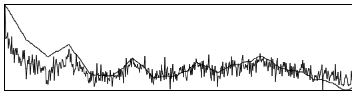
\includegraphics[clip,width=1.1\hsize]{img/POF.png}
  \caption{POF}\label{fig:POF}
\end{figure}

$$
\begin{aligned}
\mathrm{POF}[x_a, x_b]
&= \mathcal{F}^{-1}\left[\frac{\mathcal{F}\left[x_a(t)\right]^*}{|\mathcal{F}\left[x_a(t)\right]|}\mathcal{F}\left[x_b(t)\right]\right] \\
&= \mathcal{F}^{-1}\left[\frac{X_a^*(\omega)}{|X_a(\omega)|}X_b(\omega)\right]
\end{aligned}
$$


直接スペクトル拡散方式(図\ref{fig:DS})による測距システムの変復調方式を図\ref{fig:DME2}に示す.

\begin{figure}[tb]\centering
  \hspace{-2mm}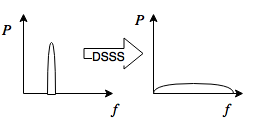
\includegraphics[clip,width=1.1\hsize]{img/DS.png}
  \caption{DS}\label{fig:DS}
\end{figure}

\begin{figure}[tb]\centering
  \hspace{-2mm}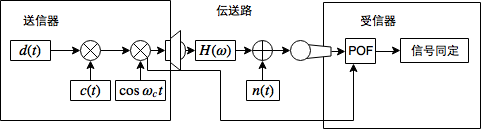
\includegraphics[clip,width=1.1\hsize]{img/DME2.png}
  \caption{DME2}\label{fig:DME2}
\end{figure}

\begin{figure}[tb]\centering
  \hspace{-2mm}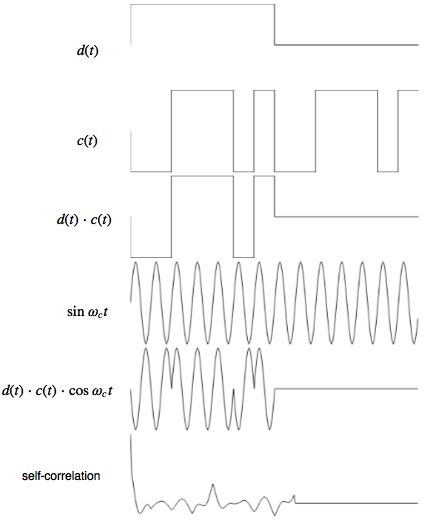
\includegraphics[clip,width=1.1\hsize]{img/DSSS.png}
  \caption{DSSS}\label{fig:DSSS}
\end{figure}

搬送波には1000Hzサイン波を,拡散符号にはM系列を用い,変調にはバイナリ位相シフトキーイング(BPSK)を使った.

復調した受信信号が雑音か有効な信号かを決定する処理を信号同定という.
伝送路における伝達関数 $H(\omega)$ において室内残響の影響
としてマルチパスによるを受けてしまう(図\ref{fig:multipath}).

\begin{figure}[tb]\centering
  \hspace{-2mm}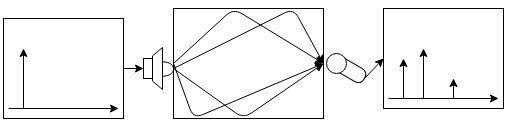
\includegraphics[clip,width=1.1\hsize]{img/multipath.png}
  \caption{multipath}\label{fig:multipath}
\end{figure}


そこで,同期パルスを測距用信号と,伝搬路を測定する参照波としてのサウンダ(sounder)信号の二つに分離した.
同期パルスから $n$ 秒後にサウンダ信号を送り,
その二つの信号の相関を取ることで,
背景雑音とは別にパルス位置を特定することが可能になる(図\ref{fig:sounder}).

\begin{figure}[tb]\centering
  \hspace{-2mm}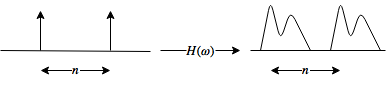
\includegraphics[clip,width=1.1\hsize]{img/sounder.png}
  \caption{sounder}\label{fig:sounder}
\end{figure}

さらにサウンダ信号と測距信号は互いに異なる同周期のM系列を用いた.
サウンダ信号と測距信号を判別しやすくするためである.

この時刻が $n$ 秒ずれた二つの信号に対して時間窓で区切って相互相関をとることで,
信号が最も相関している区間,つまり信号の位置を特定することができる.
最後に,その区間相関値を閾値処理することで信号の到来を決定する.
今回は最大相関値前方での40\%の相関値を超えたピークを到来時刻としている.

相関関数の計算にはウィーナー=ヒンチンの定理を使い周波数領域での複素乗算としてFFTを使って計算することで計算量を減らすことができる.
長さの異なる信号の高速フーリエ変換には重畳加算法\cite{overwrap}を使った.
